\documentclass[11pt,a4paper]{article}
\usepackage[T1]{fontenc}
\usepackage[utf8]{inputenc}
\usepackage{lmodern,microtype}
\usepackage[left=21mm,right=21mm,top=22mm,bottom=22mm,headheight=15pt]{geometry}
\usepackage{graphicx,xcolor,booktabs,array,longtable,tabularx}
\usepackage{listings,caption,fancyhdr,titlesec,enumitem,float}
\usepackage[hidelinks]{hyperref}
\definecolor{navy}{HTML}{12324B}
\definecolor{teal}{HTML}{0B7476}
\definecolor{muted}{HTML}{5B6874}
\definecolor{line}{HTML}{D6E0E8}
\titleformat{\section}{\Large\bfseries\color{navy}}{\thesection}{0.6em}{}
\titleformat{\subsection}{\large\bfseries\color{navy}}{\thesubsection}{0.6em}{}
\titlespacing*{\section}{0pt}{16pt}{8pt}
\setlength{\parindent}{0pt}
\setlength{\parskip}{6pt}
\setlength{\emergencystretch}{3em}
\pagestyle{fancy}
\fancyhf{}
\fancyhead[L]{\small\color{muted}CSE 472 / Web and Internet Programming Lab}
\fancyhead[R]{\small\color{muted}Lab Report 02}
\fancyfoot[L]{\small\color{muted}Jannatul Tuna Trisha / 2023200000664}
\fancyfoot[R]{\small\thepage}
\renewcommand{\headrulewidth}{0pt}
\captionsetup{font=small,labelfont=bf,skip=8pt}
\newcolumntype{L}[1]{>{\raggedright\arraybackslash}p{#1}}
\newcolumntype{Y}{>{\raggedright\arraybackslash}X}
\lstdefinelanguage{CSS}{morekeywords={color,background,margin,padding,display,grid,flex,width,height,border,font,position,media,root},sensitive=true,morecomment=[s]{/*}{*/},morestring=[b]"}
\lstdefinelanguage{JavaScript}{morekeywords={const,if,function,false,true},sensitive=true,morecomment=[l]{//},morestring=[b]",morestring=[b]'}
\lstset{basicstyle=\ttfamily\fontsize{8.5}{10.2}\selectfont,keywordstyle=\color{navy}\bfseries,
commentstyle=\color{muted},stringstyle=\color{teal},numbers=left,numberstyle=\tiny\color{muted},numbersep=8pt,
showstringspaces=false,breaklines=true,breakatwhitespace=false,columns=fullflexible,keepspaces=true,
tabsize=2,frame=single,rulecolor=\color{line},framesep=5pt,xleftmargin=12pt,xrightmargin=3pt,
aboveskip=10pt,belowskip=10pt,captionpos=t}
\newcommand{\BrowserVersion}{Chromium 143.0.7499.4}
\newcommand{\PythonVersion}{3.13.15}
\newcommand{\PlaywrightVersion}{1.57.0}
\newcommand{\SoupVersion}{4.14.3}
\newcommand{\CSSVersion}{1.5.1}
\newcommand{\PassedCount}{33}
\newcommand{\BlockedCount}{0}
\newcommand{\FailedCount}{0}
\newcommand{\TotalCount}{33}
\newcommand{\HTMLLines}{282}
\newcommand{\CSSLines}{540}

\hypersetup{pdftitle={CSE 472 Lab Report 02: HTML Fundamentals and Structured Webpage Development},pdfauthor={Jannatul Tuna Trisha}}
\begin{document}
\begin{titlepage}
\centering
{\Large\bfseries\color{navy}SOUTHEAST UNIVERSITY\par}
\vspace{8pt}
{\large Department of Computer Science and Engineering\par}
\vspace{26pt}
{\large CSE 472\par Web and Internet Programming Lab\par}
\vspace{34pt}
{\fontsize{30}{36}\selectfont\bfseries\color{navy}Lab Report 02\par}
\vspace{14pt}
{\LARGE\bfseries HTML Fundamentals and\par Structured Webpage Development\par}
\vspace{20pt}
{\small\color{muted}ASSIGNMENT TITLE\par}
\vspace{5pt}
{\large SEU Tech Event Information\par and Registration Page\par}
\vspace{32pt}
\begin{tabular}{@{}ll@{}}
\textbf{Submitted by} & Jannatul Tuna Trisha \\[8pt]
\textbf{Student ID} & 2023200000664 \\[8pt]
\textbf{Section} & 01 \\[8pt]
\textbf{Semester} & 9th \\[8pt]
\textbf{Submitted to} & Abid Ahmad \\[8pt]
\textbf{Submission date} & 8 September 2026 \\
\end{tabular}
\vfill
{\small\color{muted}Individual laboratory submission\par}
{\small\color{muted}HTML5 structure, lists, tables, forms and semantic layout\par}
\end{titlepage}
\setcounter{page}{2}

\section{Student Information}
\begin{tabularx}{\linewidth}{@{}L{36mm}Y@{}}
\toprule
Student & Jannatul Tuna Trisha \\
Student ID / Section & 2023200000664 / 01 \\
Semester & 9th \\
Department / University & Computer Science and Engineering / Southeast University \\
Course & CSE 472 -- Web and Internet Programming Lab \\
Instructor & Abid Ahmad \\
Submission date & 8 September 2026 \\
Repository folder & \url{https://github.com/Trisha105/CSE472/tree/main/labs/lab-02-html} \\
\bottomrule
\end{tabularx}
\section{Introduction}
This experiment applies the final submission task in the CSE 472 HTML lab manual: a complete single-page event information and registration website \cite{manual}. The page is titled \emph{SEU Tech Event Information and Registration Page}. Its content includes an event overview, goals, activity tracks, a four-session schedule, a registration form and contact details.

The event name, dates, sessions and rooms are classroom examples, not an official university announcement. The sample contact address comes from the manual and is labelled as an example. HTML provides the structure, an external CSS file provides the presentation, and a small JavaScript helper prevents the demonstration form from sending information.
\section{Objectives}
The aim was to build a structured HTML5 page using meaningful semantic elements and a clear heading hierarchy. The work also practised ordered, unordered and nested lists; a captioned schedule table; labelled form controls; appropriate input constraints; and correct local file paths. A further objective was to test the completed page and document its actual output with source code and browser screenshots.

\clearpage
\section{Software and Tools Used}
\begin{tabularx}{\linewidth}{@{}L{46mm}Y@{}}
\toprule
\textbf{Tool} & \textbf{Use in this experiment} \\
\midrule
UTF-8 files and command-line editing & Preserving and completing the existing HTML/CSS project. \\
\BrowserVersion & Rendering the website and exercising its controls. \\
Python \PythonVersion; Playwright \PlaywrightVersion & Automated checks and genuine browser screenshots. \\
Beautiful Soup \SoupVersion; tinycss2 \CSSVersion & Inspecting markup and parsing the stylesheet. \\
Node.js & Syntax-checking the form helper. \\
pdfLaTeX, listings and pdfinfo & Compiling the report, displaying full source code and checking PDF metadata. \\
Git and GitHub Actions & Running the actual served website, reviewing related changes and publishing the submission. \\
\bottomrule
\end{tabularx}
\section{Short Theory of HTML}
HTML stands for HyperText Markup Language. It describes the structure of webpage content and is not a general-purpose programming language. A browser reads elements such as headings, paragraphs, images, lists, tables and forms and renders them as a page. Attributes provide additional information, such as an image path, a link destination or an input type \cite{manual}.

Semantic elements describe the role of content. For example, \texttt{nav} identifies navigation, \texttt{main} contains the main page content, and \texttt{footer} holds closing information. A \texttt{div} groups a block without assigning a special semantic role, while a \texttt{span} groups a short inline part of text.
\section{HTML5 Document Structure}
The file begins with \texttt{<!DOCTYPE html>} and uses \texttt{<html lang="en">}. Its head contains UTF-8 encoding, a responsive viewport, a descriptive browser-tab title, a page description and an external CSS link. The local SVG is also used as the favicon. The deferred helper runs after the document is parsed.

The body contains a keyboard skip link, a header with exactly one \texttt{h1}, a navigation bar, a main area with five sections and a footer. About, Goals, Activities, Schedule and Registration have IDs used by the internal links. The document therefore meets the manual's requirement for at least three meaningful sections \cite{manual}.

\clearpage
\section{Important Tags and Attributes}
{\small
\begin{tabularx}{\linewidth}{@{}L{48mm}Y@{}}
\toprule
\textbf{Tag or attribute} & \textbf{Use in this implementation} \\
\midrule
\texttt{header, nav, main, section, footer} & Separate the introduction, links, main content and contact area. \\
\texttt{h1, h2, h3, p} & Give the page a main heading, section/subsection headings and paragraphs. \\
\texttt{div, span} & Group cards and fields; highlight the purpose and event details. \\
\texttt{a, href, target, rel} & Connect page anchors and external sources; safe new-tab attributes are used. \\
\texttt{img, src, alt} & Display the local event illustration with a meaningful description. \\
\texttt{ul, ol, li} & Present goals, participation steps and nested activity tracks. \\
\texttt{table, caption, thead, tbody} & Organise the table title, column headings and four session rows. \\
\texttt{tr, th, td, scope} & Define consistent rows, header associations and data cells. \\
\texttt{form, label, input, button} & Collect demonstration values and provide Submit and Reset. \\
\texttt{fieldset, legend} & Name the participation and optional-interest groups. \\
\texttt{id, for, name, value} & Associate labels, identify fields and distinguish selected choices. \\
\texttt{required, type, minlength, maxlength, pattern, min, max} & Apply native required, length, numeric-pattern, email and date constraints. \\
\bottomrule
\end{tabularx}}
\section{Requirements Analysis}
Table~\ref{tab:req} maps the manual's final task to this project. Responsive styling, a reset button, keyboard support and safe form feedback are supporting additions, not extra requirements attributed to the manual.
\begin{table}[H]\small
\caption{Final-task requirement mapping.}\label{tab:req}
\begin{tabularx}{\linewidth}{@{}L{56mm}Y@{}}
\toprule
\textbf{Requirement} & \textbf{Implemented evidence} \\
\midrule
HTML5 and semantic layout & Complete skeleton, header, nav, main, five sections and footer. \\
Meaningful headings and text & One h1, clear subheadings and explanatory event/participation content. \\
Div, span, hyperlink and image & Grouped content, highlighted text, anchors and a local SVG with alt text. \\
Three list types & Goals list, ordered steps and correctly nested activity tracks. \\
Schedule table & Caption, five column headings and four data rows. \\
Required registration controls & Name, ID, email, date, one radio group and three checkboxes. \\
Code and submission evidence & Full source, five browser screenshots, compiled report and verified ZIP. \\
\bottomrule
\end{tabularx}
\end{table}

\clearpage
\section{Project Folder Structure}
\begin{lstlisting}[numbers=none,caption={Final Lab 02 folder layout.}]
labs/lab-02-html/
|-- index.html
|-- style.css
|-- form-demo.js
|-- images/event-banner.svg
|-- screenshots/
|   |-- homepage-top.png
|   |-- event-goals.png
|   |-- event-details.png
|   |-- registration-form.png
|   `-- mobile-registration.png
|-- report/
|   |-- lab_report_02.tex
|   |-- build-metadata.tex
|   |-- test-cases.tex
|   `-- lab_report_02.pdf
|-- tests/
|   |-- results.json
|   `-- TEST_RESULTS.md
|-- build_submission.py
|-- README.md
|-- SHA256SUMS.txt
`-- CSE472_Lab_02_Complete.zip
\end{lstlisting}
The archive excludes itself, Git metadata, caches, temporary LaTeX files and unrelated repository content. SVG is used instead of the suggested JPG because it is a small scalable local image; the manual does not require a particular image format.
\section{Design and Implementation Procedure}
The repository was inspected before editing. The existing Lab 02 HTML, CSS and README on \texttt{main} were read. No other lab folder or repository-specific instruction file was present in the inspected baseline. The update retained the existing event content, section order, cards and navy/teal colour scheme.

The missing image was supplied as an original SVG, and its reference was corrected. A skip link, labelled scrollable table region, reduced-motion rule and local form feedback were added. The ID field now accepts 10--15 digits; this is an example validation rule, not a claim about university-wide ID policy.

The helper installs submission/reset handlers before enabling Submit. Native HTML validation runs first; a valid submission is then cancelled and replaced by a local demonstration message. The completed page was tested, captured in Chromium, included in this report and packaged. Only related Lab 02 files and its build workflow were intentionally changed.

\clearpage
\section{Complete HTML Source Code}
Listing~\ref{lst:html} contains all \HTMLLines{} lines of the final HTML file. Visual line wrapping in this report does not change the source.
\lstinputlisting[language=HTML,caption={Complete final index.html.},label={lst:html}]{../index.html}
\clearpage
\section{Complete CSS Source Code}
Listing~\ref{lst:css} contains all \CSSLines{} lines of the external stylesheet. The original theme is retained with small accessibility and form-state additions.
\lstinputlisting[language=CSS,caption={Complete final style.css.},label={lst:css}]{../style.css}

\clearpage
\section{Explanation of Major Website Sections}
\textbf{Header and navigation.} The header introduces the page and sample event. Six main links reach the sections and footer; a skip link and Back to top link provide additional navigation. The single main heading names the assignment.

\textbf{About and Goals.} About explains eligibility, venue and participation. The local illustration depicts a laptop and technology topics, not an actual campus photograph. Goals are shown as an unordered list, and the academic-project notice makes the fictional event status clear.

\textbf{Activities and Schedule.} An ordered list explains the demonstration process. Nested lists group Web, AI/Data and IoT/Robotics topics. The schedule has a caption, five column headings and four sample sessions. Its labelled region scrolls on narrow screens without widening the whole page.

\textbf{Registration and Contact.} Nine inputs are explicitly labelled. The four main fields use text, email and date types; radio buttons share one group name, while checkboxes allow multiple interests. The footer identifies the student and labels the manual's contact address as an example.
\subsection{Complete Safety Helper}
The helper adds no database, account system, server request or storage. Submit starts disabled, is enabled only after the handlers are installed, and remains unavailable without JavaScript. Native HTML controls supply the actual field validation \cite{standard}.
\lstinputlisting[language=JavaScript,caption={Complete form-demo.js helper.}]{../form-demo.js}

\section{Testing Procedure}
Static checks inspected explicit tag nesting, metadata, landmarks, IDs, labels, list structure, schedule rows and local file references. tinycss2 parsed the stylesheet, Chromium checked its declaration support, and Node checked the helper syntax. These are local parser/browser checks, not an official W3C conformance certificate.

The final recorded run used \BrowserVersion{} with the delivered files served by a real local HTTP server in GitHub Actions. HTML, CSS, JavaScript and the SVG were loaded through their actual URLs. The earlier local development browser had blocked direct file and loopback access; the final served-page run is a separate check and is reported independently.

Browser tests exercised required and malformed fields, date boundaries, radio exclusivity, independent checkboxes, Submit, Enter, Reset, labels, focus outlines, reduced motion and widths of 1200, 820, 390 and 320 pixels. Fictitious values were used: Demo Student, 2023000000001 and demo@example.com. The test observed the URL and network activity around submission. A separate JavaScript-disabled context checked the fallback.

External-link safety and a live visit to the HTML standard were checked separately. Any unavailable live destination is marked BLOCKED, not PASS. The university server's availability, other browser engines, physical phones and full screen-reader behaviour are not asserted. To repeat the build, install the tools in the README and run \texttt{python build\_submission.py} from the Lab 02 folder.

\section{Test Cases and Actual Results}
The final recorded run contains \TotalCount{} checks: \textbf{\PassedCount{} passed}, \textbf{\BlockedCount{} blocked}, and \textbf{\FailedCount{} failed}. The following results are generated from the executed checks. Full records are included in \texttt{tests/results.json} and \texttt{tests/TEST\_RESULTS.md}.
{\fontsize{9.5}{11.2}\selectfont
\setlength{\tabcolsep}{4pt}
\renewcommand{\arraystretch}{1.04}
\begin{longtable}{@{}L{9mm}L{34mm}L{47mm}L{69mm}@{}}
\caption{Executed tests with expected and actual results.}\label{tab:tests}\\
\toprule\textbf{ID}&\textbf{Check}&\textbf{Expected}&\textbf{Actual result}\\\midrule
\endfirsthead
\multicolumn{4}{@{}l}{Table \thetable{} continued}\\[5pt]
\toprule\textbf{ID}&\textbf{Check}&\textbf{Expected}&\textbf{Actual result}\\\midrule
\endhead
\bottomrule\endfoot
\bottomrule\endlastfoot
T01 & HTML5 structure and nesting & HTML5, metadata and balanced tags & \textbf{PASS}. Unclosed tags: 0; nesting errors: 0 \\[2pt]
T02 & Semantic structure & One h1; at least three sections; all landmarks & \textbf{PASS}. 1 main heading; 5 sections \\[2pt]
T03 & IDs and labels & Unique IDs and connected labels for every input & \textbf{PASS}. 21 IDs; 9 explicitly labelled inputs \\[2pt]
T04 & Lists & Ordered, unordered and correctly nested lists & \textbf{PASS}. 3 nested lists inside parent list items \\[2pt]
T05 & Schedule table & Caption, five headings and four consistent data rows & \textbf{PASS}. 5 headings; 4 data rows \\[2pt]
T06 & Local file references & All linked local resources exist & \textbf{PASS}. 4 references; missing: [] \\[2pt]
T07 & CSS syntax & No CSS parser errors & \textbf{PASS}. 241 declarations; 0 errors \\[2pt]
T08 & Helper syntax & Node syntax check succeeds & \textbf{PASS}. Exit code 0 \\[2pt]
T09 & Rendered image and styling & Image loaded and CSS declarations supported & \textbf{PASS}. Image loaded: True; unsupported declarations: 0 \\[2pt]
T10 & Internal navigation & Every link reaches its target & \textbf{PASS}. 8 links checked; 0 failures \\[2pt]
T11 & External link attributes & HTTPS, new tab and safe relationship attributes & \textbf{PASS}. 2 external links checked \\[2pt]
T12 & Live external destination & HTML standard loads successfully & \textbf{PASS}. HTTP 200 \\[2pt]
T13 & Required fields & Empty form rejected and first required field focused & \textbf{PASS}. Valid: False; focus: fullname \\[2pt]
T14 & Name minimum length & Two-character name rejected & \textbf{PASS}. tooShort: True \\[2pt]
T15 & Student ID limits & Letters rejected; maximum fifteen digits & \textbf{PASS}. Letter mismatch: True; capped length: 15 \\[2pt]
T16 & Email validation & Malformed email rejected & \textbf{PASS}. typeMismatch: True \\[2pt]
T17 & Date boundaries & Only 15 and 16 October accepted & \textbf{PASS}. 14, 15, 16, 17 October valid: [False, True, True, False] \\[2pt]
T18 & Radio group & Exactly one participation type selected & \textbf{PASS}. Exclusive: True \\[2pt]
T19 & Checkbox choices & Two topics can be selected independently & \textbf{PASS}. Selected topics: 2 \\[2pt]
T20 & Valid demo submission & Local confirmation; no request or navigation & \textbf{PASS}. Confirmation: True; new requests: 0 \\[2pt]
T21 & Enter-key submission & Enter uses the same safe handler & \textbf{PASS}. Unchanged URL: True; new requests: 0 \\[2pt]
T22 & Reset button & All fields and selections return to defaults & \textbf{PASS}. All controls reset: True \\[2pt]
T23 & Label interaction & Labels focus or toggle the corresponding input & \textbf{PASS}. Text focus: True; checkbox selected: True \\[2pt]
T24 & Keyboard focus & Tab gives a visible three-pixel focus outline & \textbf{PASS}. 3px solid \\[2pt]
T25 & Responsive layout at 1200px & No horizontal document overflow & \textbf{PASS}. Document width: 1200px; viewport: 1200px \\[2pt]
T26 & Responsive layout at 820px & No horizontal document overflow & \textbf{PASS}. Document width: 820px; viewport: 820px \\[2pt]
T27 & Responsive layout at 390px & No horizontal document overflow & \textbf{PASS}. Document width: 390px; viewport: 390px \\[2pt]
T28 & Responsive layout at 320px & No horizontal document overflow & \textbf{PASS}. Document width: 320px; viewport: 320px \\[2pt]
T29 & Mobile table scrolling & Wide table scrolls inside its own region & \textbf{PASS}. Horizontal offset: 100px \\[2pt]
T30 & Reduced motion & Reduced-motion preference disables smooth scrolling & \textbf{PASS}. scroll-behavior: auto \\[2pt]
T31 & No-JavaScript safety & Submit disabled; Enter sends no information & \textbf{PASS}. Disabled: True; new requests: 0; unchanged URL: True \\[2pt]
T32 & Console and page errors & No avoidable errors on the implemented page & \textbf{PASS}. Errors recorded: 0 \\[2pt]
T33 & Real resource loading & HTML, CSS, helper and SVG load through HTTP & \textbf{PASS}. All four resources returned HTTP 200: True \\[2pt]

\end{longtable}}

\clearpage
\section{Output Screenshots}
Figures~\ref{fig:home}--\ref{fig:mobile} are genuine Chromium captures of the implemented page. Four images show desktop page regions at a 1200-pixel width; the final image shows a 390-by-844-pixel mobile viewport. No screenshot is copied from the manual or recreated as a mockup.
\begin{figure}[H]\centering

\includegraphics[width=\linewidth,height=190mm,keepaspectratio]{../screenshots/homepage-top.png}
\caption{Header, navigation, introduction, local event illustration and participation details.}\label{fig:home}
\end{figure}
\clearpage
\begin{figure}[H]\centering
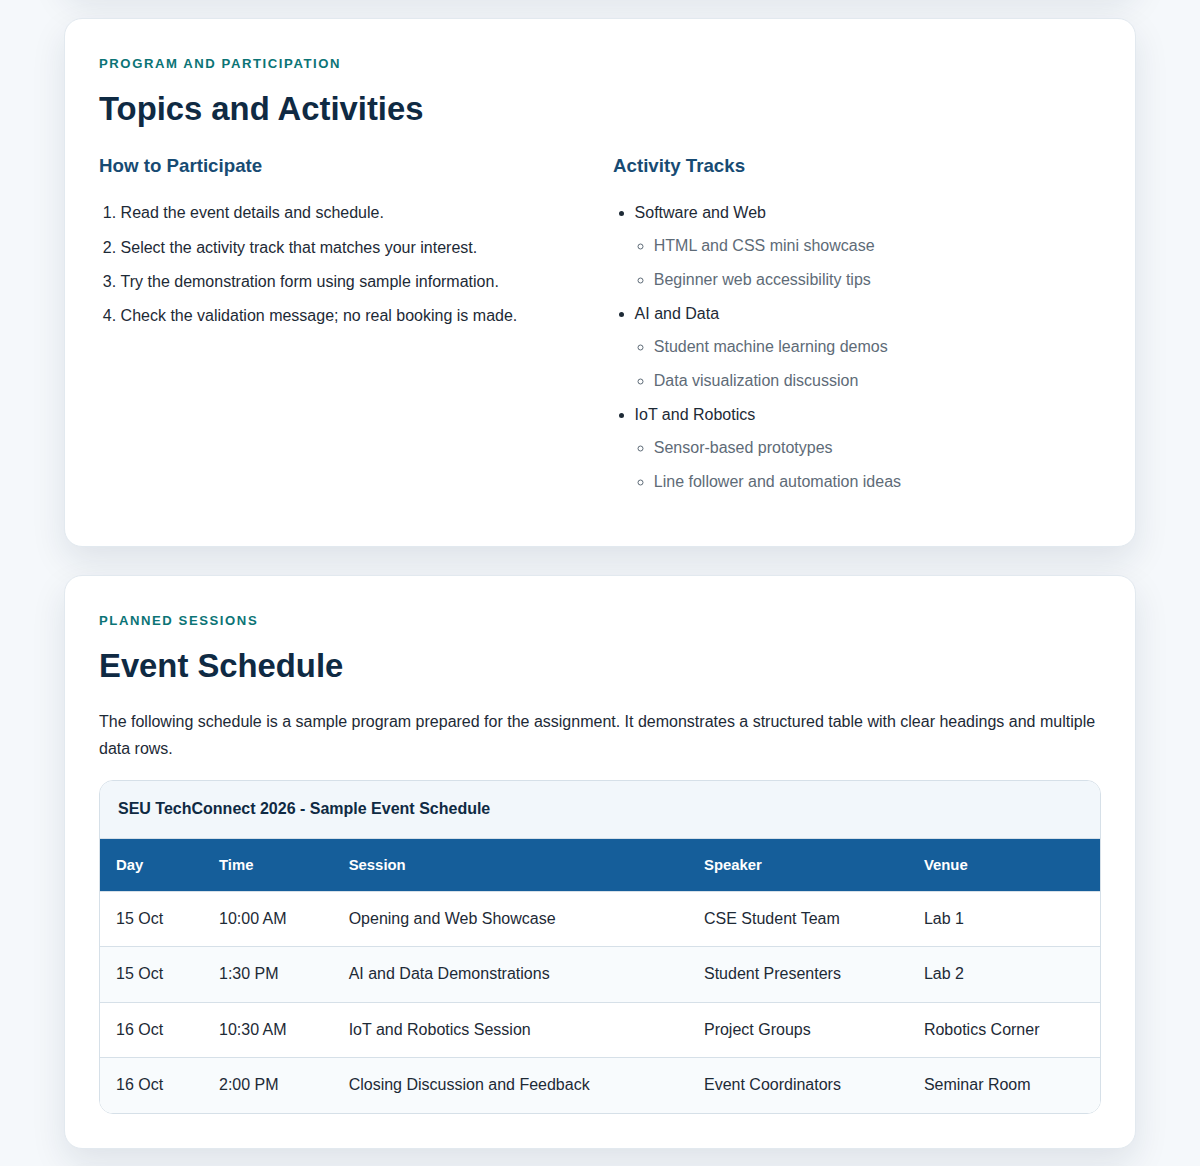
\includegraphics[width=\linewidth,height=200mm,keepaspectratio]{../screenshots/event-details.png}
\caption{Ordered participation steps, nested topic lists and the complete four-row schedule.}\label{fig:details}
\end{figure}
The activity lists are nested inside their parent items. All five headings and all four sample sessions are visible in the desktop table.
\clearpage
\begin{figure}[H]\centering
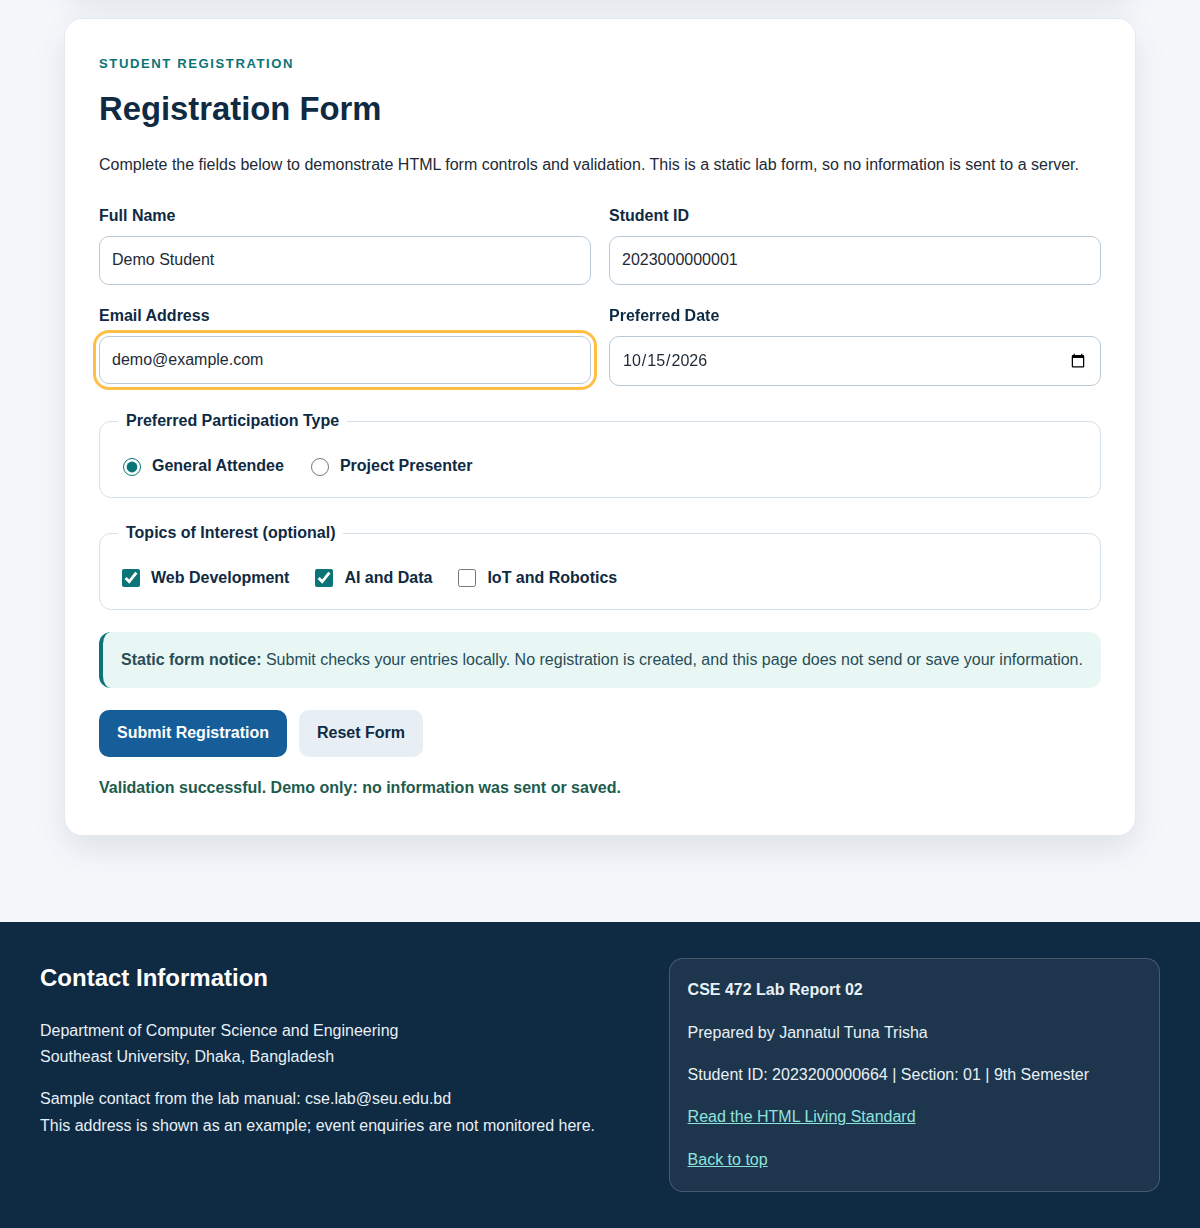
\includegraphics[width=\linewidth,height=200mm,keepaspectratio]{../screenshots/registration-form.png}
\caption{Complete form and footer after a valid demonstration submission. The fictitious test values are shown with explicit confirmation that nothing was sent or saved.}\label{fig:form}
\end{figure}
\clearpage
\begin{figure}[H]\centering
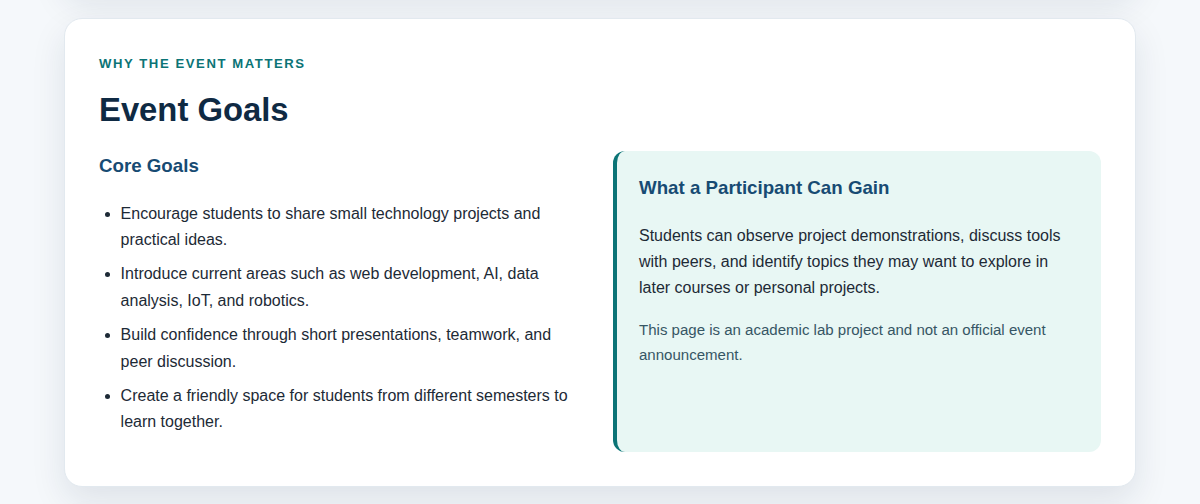
\includegraphics[width=\linewidth]{../screenshots/event-goals.png}
\caption{Unordered goals and the academic-project notice.}\label{fig:goals}
\end{figure}
\begin{figure}[H]\centering
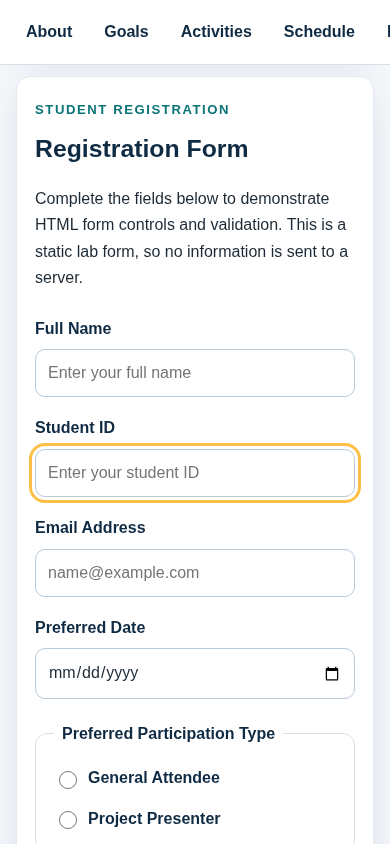
\includegraphics[height=118mm,keepaspectratio]{../screenshots/mobile-registration.png}
\caption{Mobile registration layout with one-column fields and a visible focus outline. The navigation scrolls within its own strip.}\label{fig:mobile}
\end{figure}

\clearpage
\section{Problems Faced and Solutions}
\textbf{Missing image asset.} The initial HTML referenced an event-banner JPG that was not in the repository. An original SVG was added, and the page and documentation were updated to use its real relative path. The final browser check verifies both HTTP loading and image rendering.

\textbf{A form could imply a real registration service.} The previous form silently cancelled submission. The updated version states its demonstration purpose, shows local feedback and prevents data transmission. Submit is initially disabled and stays disabled when JavaScript is unavailable. The Enter-key fallback was tested separately.

\textbf{Local browser access was restricted.} The initial development environment blocked direct file and loopback navigation. A browser-preview run was used during development. The final suite runs in GitHub Actions against a real HTTP server, so resource loading is not inferred only from files existing on disk.

\textbf{Long source listings needed readable page layout.} The report includes the actual final files through \texttt{listings}, with wrapping and line numbers. Screenshots preserve aspect ratio. Repeated table headings keep the test cases readable across pages.
\section{Learning Outcomes}
The work shows how individual HTML elements combine into a complete page. Label-click and keyboard tests demonstrate the relationship between an input and its label. Goals and steps are suited to lists, while a schedule needs consistent table headings and rows. Separating HTML and CSS keeps the document structure clear while allowing responsive layouts.

The form also demonstrates an important limitation: visible input controls and browser validation do not create a registration service. A production version would require a backend, server-side validation and an appropriate data-handling process. Recording blocked checks separately from successful tests is part of reporting results accurately.
\clearpage
\section{Conclusion}
The Lab 02 page combines the required HTML5 structure, semantic sections, meaningful text, links, image, lists, schedule and registration controls. The existing design was completed without changing another lab. The actual browser results document the tested behaviour and distinguish any unavailable external check. Complete source code, five screenshots, the compiled report, reproducible build script and a verified ZIP are included in the submission.
\section{References}
\begingroup\renewcommand{\section}[2]{}
\begin{thebibliography}{9}
\bibitem{manual} A. Ahmad, \emph{CSE 472 -- Web and Internet Programming Lab: Complete HTML Lab Manual}, Southeast University. Supplied course manual, especially Sections 19--26. The uploaded copy was a DOCX document.
\bibitem{standard} WHATWG, \emph{HTML Living Standard}. Accessed 8 September 2026. \url{https://html.spec.whatwg.org/multipage/}
\end{thebibliography}\endgroup
\textbf{Image attribution:} \texttt{images/event-banner.svg} is an original illustration created for this submission using simple vector shapes and text. It is not a campus photograph and contains no third-party logo or font file. The five output images are browser captures of this project.
\end{document}
